\begin{center}
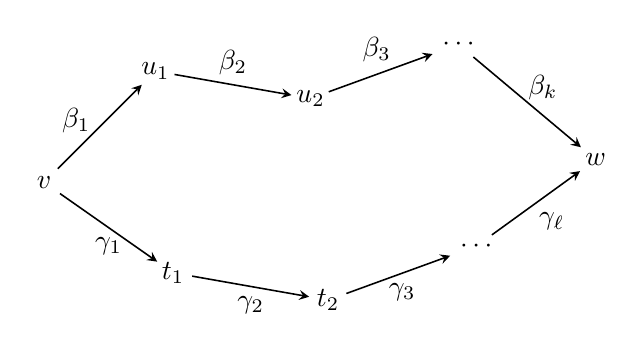
\begin{tikzpicture}[line width = 0.2mm, >=stealth, shorten >= 7pt, shorten <=7pt]
\draw[->, Black] (0,0) coordinate (a)
-- node[above, xshift = -0.3cm, yshift = -0.2cm] {$\beta_1$} ++(45:2) coordinate (b);
\draw[->, Black,] (b)
-- node[above] {$\beta_2$} ++(-10:2) coordinate (c);
\draw[->, Black, shorten >= 10pt] (c)
-- node[above, xshift = -0.1cm] {$\beta_3$} ++(20:2) coordinate (d);
\draw[->, Black] (d)
-- node[above, xshift = 0.2cm, yshift = -0.1cm] {$\beta_k$}++(-40:2.275) coordinate (e);
\node[] at (a) {$v$};
\node[] at (b) {$u_1$};
\node[] at (c) {$u_2$};
\node[] at (d) {$\cdots$}; 
\node[] at (e) {$w$};

\draw[->, Black] (0,0)
-- node[below] {$\gamma_1$}++(-35:2) coordinate (f);
\draw[->, Black] (f)
-- node[below] {$\gamma_2$}++(-10:2) coordinate (g);
\draw[->, Black, shorten >= 10pt] (g)
-- node[below] {$\gamma_3$}++(20:2) coordinate (h);
\draw[->, Black] (h)
-- node[below, xshift = 0.2cm] {$\gamma_{\ell}$} (e);
\node[] at (f) {$t_1$};
\node[] at (g) {$t_2$};
\node[] at (h) {$\cdots$};
\end{tikzpicture}
\end{center}